% !TEX encoding = UTF-8
% !TEX TS-program = pdflatex
% !TEX root = ../tesi.tex

%**************************************************************
\chapter{Il progetto nella strategia aziendale}
\label{cap:processi-metodologie}
%**************************************************************

\section{Azienda e stage}
%Lab Network Srl è solita ospitare tirocinanti e stagisti per dare loro una formazione e valutarne le capacità per un possibile inserimento in azienda.

Lab Network Srl è solita ospitare tirocinanti e stagisti per lunghi o brevi periodi e da quest'anno è stato stipulato l'accordo con l'Università di Padova che consente all'azienda di ospitare anche studenti universitari.

% Approfondimento dell'eventuale pregresso (esperienza e risultati) dell'azienda con stage precedenti di ambito INF
Le passate esperienze con altri studenti consistevano principalmente nella creazione di siti web, perché il tempo a disposizione era inferiore a quello a me concesso. Ad ogni modo, nonostante il carico di lavoro fosse minore, hanno soddisfatto la clientela dando a \lab{}.

Il tirocinio è vantaggioso sia per l'azienda che per lo stagista:
\begin{itemize}
\item \textbf{Dal punto di vista aziendale}: ospitare uno studente, o in generale una persona, per un periodo all'interno di un progetto di stage, consente all'azienda di valutare le capacità lavorative dello stagista e, se quest'ultimo risulta valido, considerare il tirocinio come un periodo di formazione finalizzato all'assunzione.

Lo stage, inoltre, consente di portare a compimento alcuni progetti non troppo complessi, catalogati come secondari, che fino a quel momento non avevano trovato spazio all'interno dell'azienda.
\item \textbf{Dal punto di vista dello studente}: uno stage è un'ottima opportunità per mettere in pratica quanto appreso durante gli studi; inoltre, spesso consente di accrescere la propria formazione, perché si presenta la necessità dell'utilizzo di nuove tecnologie e nuovi strumenti di lavoro.
\end{itemize}

%Il tirocinio porta un vantaggio sia per gli stagisti stessi, che hanno modo di mettere in pratica in campo lavorativo quanto appreso durante gli studi, sia per l'azienda che ha modo di valutare le capacità di una persona al fine dell'assunzione formandola al tempo stesso. 

%Alcuni progetti classificati come non prioritari, spesso non trovano spazio all'interno dell'azienda, che decide quindi di farne oggetto di stage.

\medskip

Sono venuto a conoscenza di Lab Network grazie alla diffusione mediatica di alcuni loro progetti che stavano avendo successo, come ad esempio Vitruvian Game, e così ho deciso di propormi all'azienda per lo svolgimento del tirocinio: quest'ultima ha accettato proponendomi alcuni progetti disponibili tra cui FabKey.

%Lab Network ha deciso di portare avanti questo progetto attraverso uno stage, perché fino ad allora era stato catalogato come secondario e non aveva ancora trovato il suo spazio all'interno dell'azienda.

\medskip

FabKey è stato proposto come progetto di stage, in quanto era stato fino ad allora catalogato come secondario e non aveva ancora trovato il suo spazio all'interno dell'azienda. Per di più, coinvolgere uno studente universitario nello sviluppo del progetto, sarebbe stato vantaggioso sfruttando le capacità che lo stagista ha sviluppato durante il corso di studi.

\section{Obiettivi aziendali}
L'obiettivo principale del progetto di stage è l'ampliamento del già collaudato sistema ``FabKey'', il quale permette l'apertura di una porta attraverso un tag NFC controllando una lista di accessi presente in un database online. Nello specifico, tale sistema doveva essere revisionato e ampliato, utilizzando un modulo che andrà ad autenticare l'utente tramite codice a barre anziché tag NFC.

Gli obiettivi concordati con il tutor aziendale sono stati classificati secondo tre gradi di priorità:

\begin{enumerate}
\item \textbf{Obbligatori}: obiettivi il cui sviluppo è necessario per la riuscita del progetto;
\begin{itemize}
\item \textbf{Integrazione di un sistema completo per l'apertura di serrature con lettura di codice a barre e NFC.} L'obiettivo principale richiesto dall'azienda è quello di ampliare il sistema esistente, che consiste in una centralina di controllo e di un modulo NFC, con un modulo per la lettura di codici a barre. Si rende necessaria la riprogrammazione della centralina, aggiungendo la nuova parte di codice per la gestione dei codici a barre; 
\item \textbf{Realizzazione della piattaforma web per la gestione degli accessi.} La piattaforma web per il controllo degli accessi è uno strumento indispensabile per l'utilizzo del sistema FabKey, pertanto la sua realizzazione è un requisito obbligatorio. Questa applicazione web sarà composta da un pannello di controllo che permette l'utente di modificare le autorizzazioni d'accesso a uno o più varchi e di consultare un report contenente tutti gli accessi effettuati; 
\item \textbf{Creazione del modello 3D dell'involucro e sua realizzazione con stampa 3D.} Durante la definizione degli obiettivi è stato accordato che tutta la parte elettronica sarà inserita in un involucro disegnato su misura e stampato in 3D; 
\item \textbf{Redazione della manualistica completa.} A corredo del kit, all'utente finale sarà consegnata tutta la manualistica necessaria all'installazione e all'uso. Sono necessari anche dei manuali interni per la guida all'assemblaggio, alla codifica e alla corretta configurazione per il cliente finale;
\end{itemize}

\medskip

\item \textbf{Desiderabili}: il loro sviluppo non è necessario ai fini del progetto, ma forniscono un valore aggiunto considerevole;
\begin{itemize}
\item \textbf{Cura e definizione dell'interfaccia grafica della piattaforma web.} Seppur trattandosi di un aspetto non vincolante ai fini del progetto, una grafica curata accresce in modo significativo il valore del prodotto finale;
\item \textbf{Ottimizzazione del sistema esistente in termini di efficienza e prestazioni}. Con questo obiettivo si vogliono ridurre i tempi di risposta dell'intero sistema, ottimizzando l'esecuzione del codice in generale e in particolare le chiamate HTTP al server; 
\end{itemize}

\medskip

\item \textbf{Facoltativi}: il loro sviluppo diventa apprezzabile, ma dal valore aggiunto trascurabile.
\begin{itemize}
\item \textbf{Creazione di un modello 3D modulare espandibile per future versioni}. In previsione di future espansioni con l'utilizzo di elettronica differente, è apprezzabile la creazione del modello 3D in modo modulare e universale, compatibile quindi con eventuali modifiche future. 
\end{itemize}
\end{enumerate}

\begin{figure}[H]
	\begin{center}
	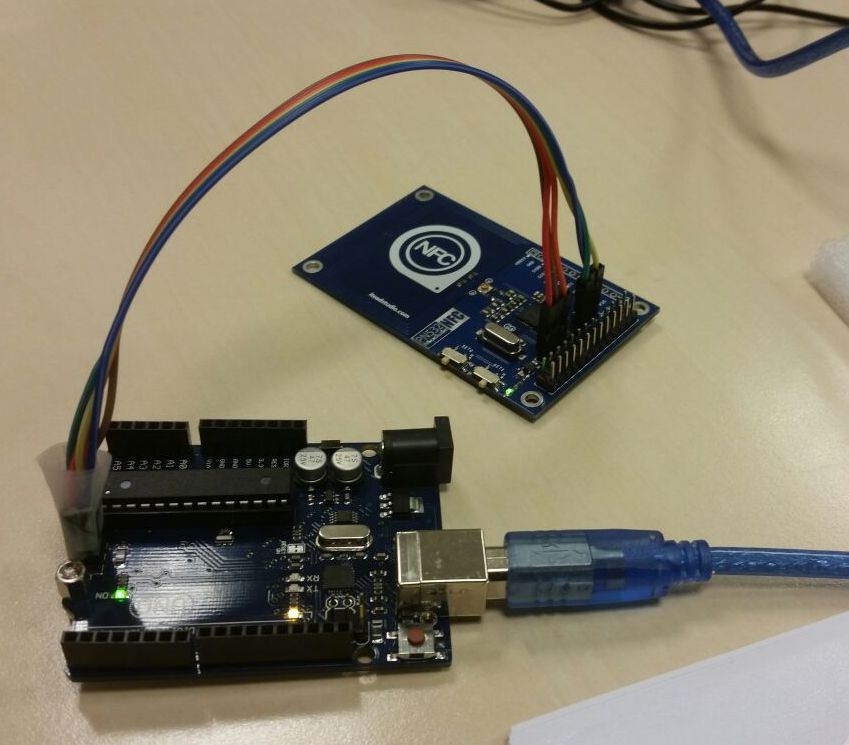
\includegraphics[scale=0.25]{immagini/fabkey_prima.jpg}
	\caption{Prototipo funzionante di FabKey prima dell'inizio dello stage.}
	\end{center}
\end{figure}

La realizzazione di questo progetto può portare diversi vantaggi a \lab{} tra cui:

\begin{itemize}
\item Grazie all'immissione sul mercato di FabKey, l'azienda ha l'opportunità di entrare nel mercato consumer, ampliando così il tipo di clientela. Data la semplicità di installazione e configurazione, il prodotto finito potrà essere venduto anche a clienti privati;

\item La fornitura prevista a tutti i FabLab del territorio fa si che il prodotto si diffonda sin dalla prima immissione sul mercato.
\end{itemize}

\begin{figure}[H]
	\begin{center}
	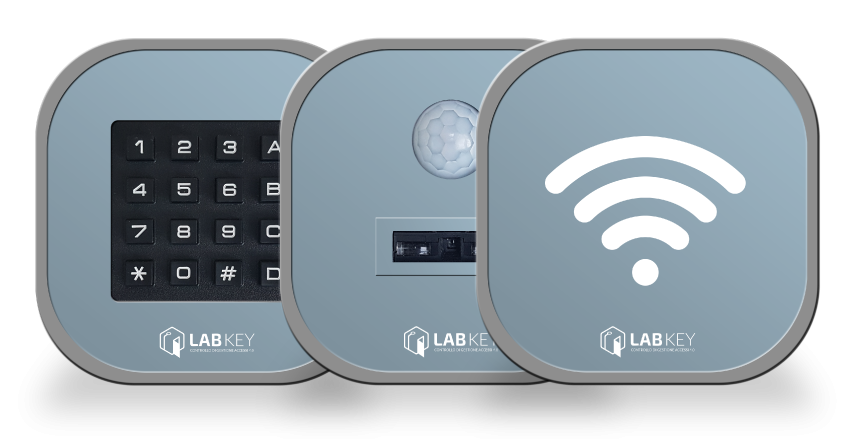
\includegraphics[scale=0.3]{immagini/fabkey_dopo.png}
	\caption{Il prodotto finito dopo il termine dello stage.}
	\end{center}
\end{figure}

\section{Vincoli}
Mi sono stati imposti dei vincoli da parte dell'azienda in termini di tempo e tecnologie, al fine di un corretto svolgimento del progetto oltre che una buona integrazione con il resto del team di sviluppo. 

Quanto stabilito a monte dello stage, è stato trascritto all'interno di un piano di lavoro, redatto in collaborazione con il tutor aziendale.

I vincoli tecnologici sono:
\begin{itemize}
\item \textbf{GitLab}: si tratta di una piattaforma web per la gestione di repository Git. Mi è stato chiesto di utilizzare questo strumento anche per la gestione di ticket e del Product Backlog;
\item \textbf{Arduino IDE}: applicazione che consente la programmazione di schede Arduino e compatibili. Viene fornito con un editor di testo, un compilatore e una serie di esempi per ogni libreria disponibile. Utilizzando schede Arduino per la gestione dei moduli NFC e barcode, risulta necessario l'utilizzo di questo ambiente;
\item \textbf{Rhinoceros}: mi è stato chiesto, dopo un'adeguata documentazione, di utilizzare questo software per per la modellazione dell'involucro contenente l'elettronica di FabKey.
\end{itemize}

\begin{figure}[H]
	\begin{center}
	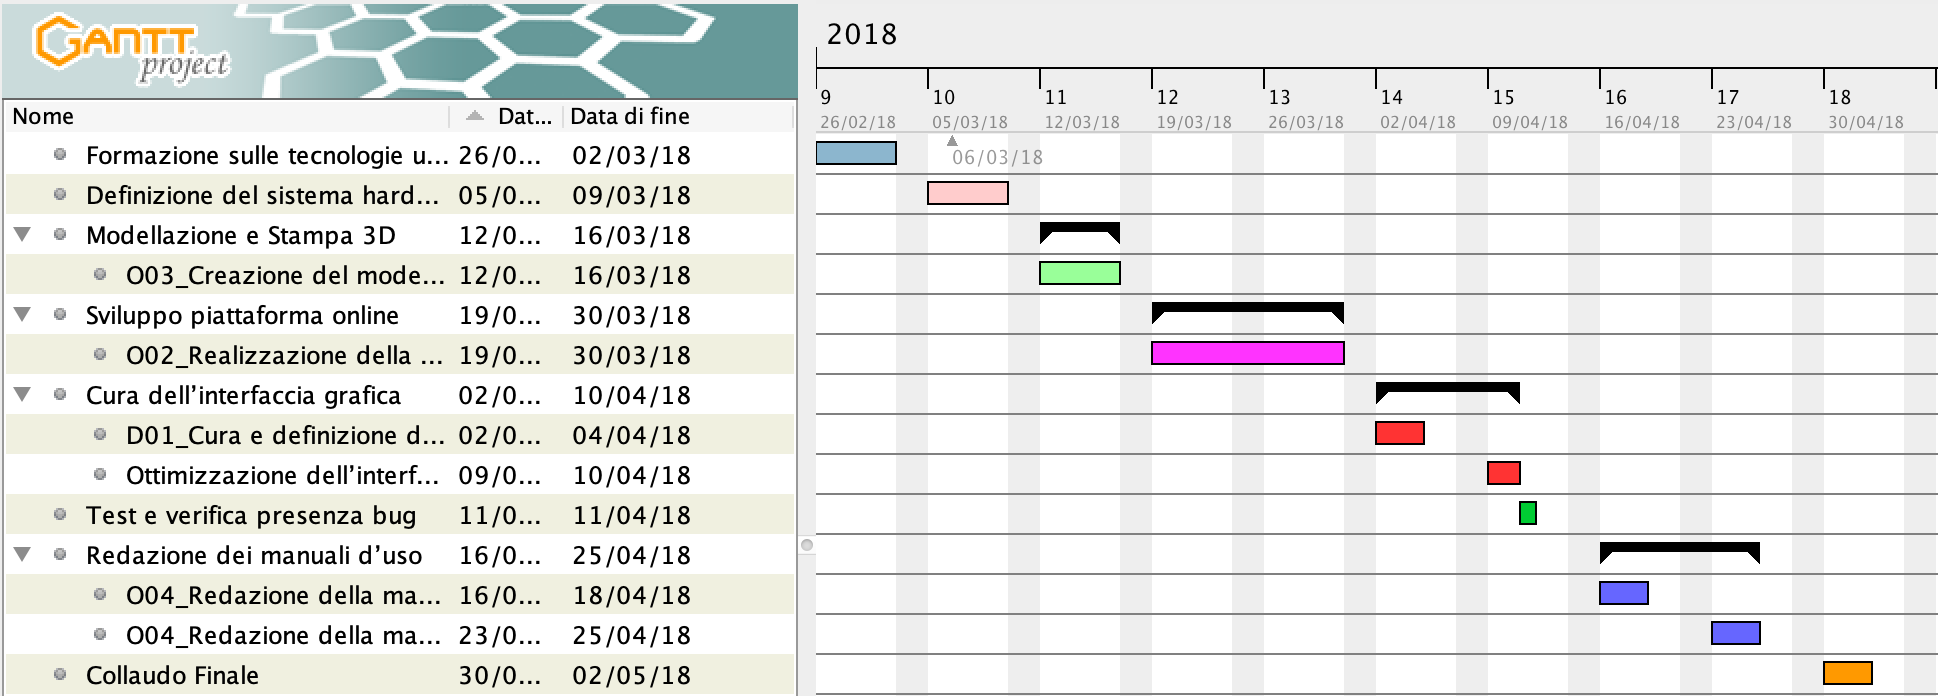
\includegraphics[scale=0.4]{immagini/gantt.png}
	\caption{Diagramma di Gantt per la pianificazione del progetto di stage.}
	\end{center}
\end{figure}

Il tempo a disposizione per lo svolgimento del tirocinio è di almeno 300 ore, le quali sono state suddivise in 40 ore settimanali per le prime 5 settimane e le rimanenti ore suddivise su una base di 24 ore settimanali.

\medskip

Al termine dello stage, sono stati tralasciati alcuni degli obiettivi tra i desiderabili e i facoltativi principalmente per mancanza di tempo.
Per migliorare il prodotto, ho ricevuto la proposta da parte del tutor di continuare a lavorare nella sua azienda.

\section{Obiettivi personali}
Le motivazioni che mi hanno spinto a scegliere questo progetto presso \lab{} sono:

\begin{itemize}
\item \textbf{Codifica e correlazione tra hardware e software}: un aspetto dell'informatica che mi ha da sempre affascinato è l'interazione tra hardware e software; non avendo potuto approfondire l'argomento durante gli studi, ho trovato questa proposta di stage un'ottima opportunità per studiare sul campo la programmazione hardware. Il progetto, inoltre, si affaccia al mondo dell'\textit{Internet Of Things} che è in continua crescita;
\item \textbf{Modellazione e stampa 3D}: è un campo molto diffuso e in continua crescita. Con questo progetto di stage mi è stata offerta la possibilità di usare in esclusiva una stampante 3D per la realizzazione dei primi prototipi dopo averli correttamente modellati;
\item \textbf{Lavoro in team}: fare parte di un team di sviluppo cogliendo gli aspetti in comune e le differenze tra un progetto accademico come quello svolto durante il corso di Ingegneria del Software e un progetto in ambito lavorativo. 
\end{itemize}

Le mie aspettative nello svolgimento di questo progetto di stage erano principalmente:
\begin{itemize}
\item \textbf{Formazione lavorativa in ambito software}: il mio interesse era di poter vivere un'esperienza lavorativa presso un'azienda del settore ICT, mettendola a confronto con i miei precedenti impieghi presso aziende di altri settori;
\item \textbf{Accrescere le mie conoscenze}: apprendere velocemente sul campo sia mettendo in pratica quanto appreso durante di studi che utilizzando nuove tecnologie e nuovi strumenti.
\end{itemize}


